% !TEX program = pdflatex
\documentclass[journal]{IEEEtran}

% === Packages ===
\usepackage{cite}
\usepackage{amsmath,amssymb,amsfonts}
\usepackage[ruled,vlined,linesnumbered]{algorithm2e}
\usepackage{xspace}
\usepackage{graphicx}
\usepackage{textcomp}
\usepackage{xcolor}
\usepackage{booktabs}
\usepackage{multirow}
\usepackage{subcaption}
\usepackage{url}
\usepackage{balance}
\usepackage{tikz}
\usetikzlibrary{positioning,arrows.meta,shapes.geometric,fit,backgrounds,calc}

\graphicspath{{figures/}}

% === Custom commands ===
\newcommand{\eg}{\textit{e.g.}\xspace}
\newcommand{\ie}{\textit{i.e.}\xspace}
\newcommand{\etal}{\textit{et al.}\xspace}
\newcommand{\QtoC}{\textsc{Q2C}\xspace}
\newcommand{\R}{\mathbb{R}}
\newcommand{\bK}{\mathbf{K}}
\newcommand{\bV}{\mathbf{V}}
\newcommand{\bQ}{\mathbf{Q}}
\newcommand{\bA}{\mathbf{A}}

\begin{document}

\title{Scout: Cross-Model Attention Transfer for\\Bandwidth-Adaptive Edge-Cloud LLM Inference}

\author{
\IEEEauthorblockN{Wei-Lun~Cheng and Wanjiun~Liao,~\IEEEmembership{Fellow,~IEEE}}
\IEEEauthorblockA{Department of Electrical Engineering,
National Taiwan University, Taipei, Taiwan\\
\{d11921b15, wjliao\}@ntu.edu.tw}
\thanks{Manuscript received XX, 2026. This work was supported in part by the National Science and Technology Council, Taiwan.}
}

\maketitle

% ============================================================
% ABSTRACT
% ============================================================
\begin{abstract}
Edge-cloud LLM inference requires transmitting key-value (KV) cache states over bandwidth-limited wireless links---a 14B model's cache exceeds 200\,MB at 1024 tokens.
We propose \emph{Scout}, which eliminates KV-cache transmission by exploiting attention alignment within model families: a small edge model's query-to-context attention scores identify the same task-relevant positions as the cloud model (84--92\% overlap across three architectures, $n\!=\!200$, $p > 0.06$), reducing payload from 9.7\,MB to 336~bytes---a 28{,}800$\times$ compression.
We design a bandwidth-adaptive protocol with five modes that dynamically selects compression strategy using real 5G traces, achieving 100\% deadline compliance via scout fallback.
Characterization across 7~models from 5~families shows INT8 is universally lossless, INT4 fragility is model-specific, and \QtoC selection matches SnapKV while outperforming H2O.
For 2--8 agents sharing a base station, model-aware allocation converts 0\% to 100\% deadline compliance under congestion.
\end{abstract}

\begin{IEEEkeywords}
Collaborative inference, KV-cache, cross-model attention, adaptive protocol, edge-cloud computing, large language models
\end{IEEEkeywords}

% ============================================================
% I. INTRODUCTION
% ============================================================
\section{Introduction}
\label{sec:intro}

The deployment of large language models (LLMs) in distributed environments is driving interest in \emph{collaborative inference}, where computational stages are split across edge and cloud devices~\cite{splitwise,distserve}.
In this architecture, an edge device performs the \emph{prefill} pass---encoding the user's context and query---while a cloud server with greater compute capacity executes the \emph{decode} pass, generating tokens autoregressively.
The key-value (KV) cache produced during prefill must be transmitted to the cloud, creating a bandwidth bottleneck.

For a representative 14B-parameter model (Qwen2.5-14B: 48~layers, 8~KV heads, 128~head dimension), a 1024-token context produces a KV-cache of size $2 \times 48 \times 8 \times 1024 \times 128 \times 2 \approx 201$\,MB in BF16.
At 100\,Mbps---typical for 5G uplink---this requires $\sim$16 seconds of transmission latency, clearly impractical for interactive applications.
Even a 7B model (Qwen2.5-7B: 28~layers, 4~KV heads) generates 58\,MB at 1024~tokens, requiring 4.6~seconds.
At lower bandwidths common in edge deployments (10--50\,Mbps), latency becomes prohibitive.

Existing approaches address this bottleneck along narrow dimensions.
CacheGen~\cite{cachegen} applies delta encoding and layer-wise quantization with arithmetic coding, achieving $\sim$3.5$\times$ compression.
H2O~\cite{h2o} and SnapKV~\cite{snapkv} perform token eviction using attention-based importance scores.
KIVI~\cite{kivi} and KVQuant~\cite{kvquant} study pure quantization.
However, all these methods treat compression as a static, single-model problem and do not adapt to time-varying wireless conditions.

We make a key observation that enables a fundamentally different approach: \emph{models within the same family attend to similar context positions}.
Across three architectures---Qwen~2.5 (7B$\to$14B), Llama~3 (3B$\to$8B), and Gemma~2 (2B$\to$9B)---a small model's query-to-context attention scores produce position selections that overlap 84--92\% with the larger model's selections at 75\% retention.
This enables a \emph{scout model} paradigm: the lightweight edge model identifies important positions, transmits only the position indices (336~bytes instead of 9.7\,MB), and the cloud model applies this selection to its own KV-cache---a 28{,}800$\times$ payload reduction versus CacheGen's 3.5$\times$.

This paper makes four contributions:

\begin{enumerate}
    \item \textbf{Scout protocol}: We propose transmitting position indices instead of KV-cache data, achieving 28{,}800--98{,}800$\times$ payload reduction. We validate across three model families: Qwen~2.5 (83.7\% overlap, $p = 0.88$), Llama~3 (91.8\%, $p = 0.06$), and Gemma~2 (86.1\%, $p = 0.36$), all at 75\% retention with $n = 200$---confirming that cross-model attention alignment is architecture-general.

    \item \textbf{Bandwidth-adaptive 5-mode protocol}: We design a protocol engine that dynamically selects among full-KV, INT8, INT4, mixed-INT4, and scout modes based on real-time channel conditions. Using real 5G network traces, the adaptive policy achieves 98--107\% quality with up to 100\% deadline compliance.

    \item \textbf{Multi-agent model-aware allocation}: For $N$ edge devices sharing bandwidth, model-aware allocation converts 0\% deadline compliance to 100\% under congestion, scaling to 8~agents.

    \item \textbf{KV-cache compressibility characterization}: Through systematic evaluation across 5~model families ($n = 200$ each), we show that INT8 is universally lossless, INT4 fragility is model-specific, and \QtoC selection matches SnapKV (both significantly outperform H2O at aggressive retention). Perplexity validation on WikiText-2 confirms: INT4 is catastrophic for sensitive models (PPL~80.3 vs.~8.6 baseline).
\end{enumerate}

Our approach differs fundamentally from prior KV-cache compression work.
Methods such as CacheGen~\cite{cachegen}, H2O~\cite{h2o}, and SnapKV~\cite{snapkv} compress the KV-cache data itself, achieving 2--4$\times$ reduction.
Scout eliminates the need to transmit KV data altogether by transferring only the \emph{positions} where the cloud should attend, achieving 28{,}800$\times$ reduction.
This is conceptually similar to speculative decoding~\cite{speculativedecoding}, where a small model guides a larger one---but applied to \emph{position selection} rather than \emph{token generation}, and motivated by bandwidth reduction rather than latency reduction.

The remainder of this paper is organized as follows. Section~\ref{sec:system} presents the system model and problem formulation. Section~\ref{sec:attention} analyzes cross-model attention alignment---the theoretical and empirical foundation of the scout approach. Section~\ref{sec:protocol} describes the scout protocol design, including mode selection, hybrid mode, and multi-turn extensions. Section~\ref{sec:compression} characterizes KV-cache compression operating points across models, tasks, and quantization strategies. Section~\ref{sec:transport} presents the adaptive transport protocol and multi-agent allocation. Section~\ref{sec:experiments} provides comprehensive experimental evaluation with $n = 200$ samples and statistical rigor. Section~\ref{sec:related} surveys related work. Section~\ref{sec:conclusion} concludes.


% ============================================================
% II. SYSTEM MODEL AND PROBLEM FORMULATION
% ============================================================
\section{System Model and Problem Formulation}
\label{sec:system}

\subsection{Edge-Cloud Architecture}

We consider $N$ edge devices $\{E_1, \ldots, E_N\}$ sharing a wireless uplink to a cloud server~$C$.
Each edge device~$E_i$ runs a lightweight model~$M_i^{\text{edge}}$ (\eg, 3B--7B parameters), while the cloud runs a larger model~$M^{\text{cloud}}$ (\eg, 7B--14B parameters).
Both models belong to the same family, sharing the tokenizer and positional encoding scheme (RoPE with identical base frequency).
The total uplink bandwidth $B_{\text{total}}(t)$ is time-varying and shared among active devices.

The inference pipeline proceeds in four phases:
\begin{enumerate}
    \item \textbf{Edge prefill}: Device~$E_i$ receives context tokens $\mathcal{C} = \{c_1, \ldots, c_n\}$ and query tokens $\mathcal{Q} = \{q_1, \ldots, q_m\}$, runs the prefill forward pass to produce $\bK^e, \bV^e$ and attention weights $\bA^e$.
    \item \textbf{Compression}: The edge applies compression function $\phi$ to produce a compact representation $Z = \phi(\bK^e, \bV^e, \bA^e)$.
    \item \textbf{Transmission}: $Z$ is transmitted over the wireless uplink to the cloud.
    \item \textbf{Cloud decode}: The cloud decompresses $Z$ (or, in scout mode, runs its own prefill with the received position mask) and generates the response autoregressively.
\end{enumerate}

The key design variable is the compression function $\phi$, which determines the tradeoff between transmission payload $|Z|$ and task quality $Q(\phi)$.

\subsection{KV-Cache Structure}

For a transformer model with $L$ layers, $H$ KV-heads per layer, head dimension $d$, and sequence length $n$, the KV-cache consists of:
\begin{equation}
    \bK, \bV \in \R^{L \times H \times n \times d}
\end{equation}
In BF16 precision, the total KV-cache size is $2LHnd \times 2$ bytes.
Table~\ref{tab:models} lists the models evaluated in this work with their KV-cache sizes.

\begin{table}[t]
\centering
\caption{Models evaluated (9 models, 5 families) with KV-cache sizes at 1024 tokens in BF16.}
\label{tab:models}
\small
\begin{tabular}{@{}lccccc@{}}
\toprule
\textbf{Model} & \textbf{Params} & \textbf{Layers} & \textbf{KV-H} & \textbf{KV@1K$^\dagger$} \\
\midrule
Qwen2.5-3B       & 3B   & 36 & 2  & 18.9\,MB \\
Qwen2.5-7B       & 7B   & 28 & 4  & 29.4\,MB \\
Qwen2.5-14B      & 14B  & 48 & 8  & 100.7\,MB \\
Llama-3.2-3B     & 3B   & 28 & 8  & 58.7\,MB \\
Llama-3.1-8B     & 8B   & 32 & 8  & 67.1\,MB \\
Gemma-2-2B$^*$   & 2B   & 26 & 4  & 54.5\,MB \\
Gemma-2-9B$^*$   & 9B   & 42 & 8  & 176.2\,MB \\
Mistral-7B-v0.3  & 7B   & 32 & 8  & 67.1\,MB \\
Yi-1.5-6B        & 6B   & 32 & 4  & 33.6\,MB \\
\bottomrule
\multicolumn{5}{@{}l}{\scriptsize $^\dagger$Per-direction (K or V); full KV-cache is $2\times$.} \\
\multicolumn{5}{@{}l}{\scriptsize $^*$Gemma-2 uses 256 head dim (others: 128).}
\end{tabular}
\end{table}

\subsection{Operating Modes}

We identify five operating modes with decreasing bandwidth requirements:

\begin{table}[t]
\centering
\caption{Operating modes with quality and bandwidth characteristics (Qwen-7B, SQuAD~v2, $n = 200$, $\sim$170 avg.\ context tokens).}
\label{tab:operating_points}
\small
\begin{tabular}{@{}lccc@{}}
\toprule
\textbf{Mode} & \textbf{Payload} & \textbf{Quality} & \textbf{TX@100Mbps} \\
\midrule
Full BF16       & 9.7\,MB   & 100\%  & 775\,ms \\
INT8            & 4.7\,MB   & 99.4\% & 388\,ms \\
INT4            & 2.3\,MB   & 68.7\% & 195\,ms \\
Mixed INT4      & 2.6\,MB   & 93.6\% & 216\,ms \\
Scout (indices) & 336\,B    & $\sim$100\%$^\dagger$ & 0.03\,ms \\
\bottomrule
\end{tabular}
\end{table}

\noindent\emph{Note:} $^\dagger$Scout quality depends on model pair; 7B$\to$14B achieves 99.4\% at 75\% retention.

\subsection{Problem Formulation}

Given time-varying bandwidth $B(t)$, a quality-of-service (QoS) deadline $T_{\max}$, and $N$ concurrent requests, we seek:
\begin{equation}
    \max_{\pi} \; \mathbb{E}\left[\sum_{i=1}^{N} Q_i(\pi_i(B_i(t)))\right]
    \label{eq:objective}
\end{equation}
\vspace{-2mm}
\begin{equation}
    \text{s.t.} \quad \sum_{i=1}^{N} B_i(t) \leq B_{\text{total}}(t), \quad T_i \leq T_{\max} \; \forall i
\end{equation}
where $\pi_i$ is the operating mode selection policy for device~$i$, $Q_i$ is the task quality, $B_i(t)$ is the bandwidth allocated to device~$i$, and $T_i$ is the end-to-end latency including prefill, quantization, transmission, and decode.

The compression ratio for a combined pipeline is:
\begin{equation}
    \rho = r \times \frac{\bar{b}}{16}, \quad \bar{b} = \frac{1}{L}\sum_{l=1}^{L} b^{(l)}
\end{equation}
where $r$ is the token retention ratio and $\bar{b}$ is the average bit-width across layers.

Fig.~\ref{fig:system} illustrates the Scout architecture.
The edge device runs a lightweight model to score token positions via \QtoC, then the protocol engine selects among five operating modes based on current bandwidth.
In scout mode, only position indices traverse the wireless link; the cloud re-prefills with its own model and applies the received mask.

\begin{figure*}[t]
\centering
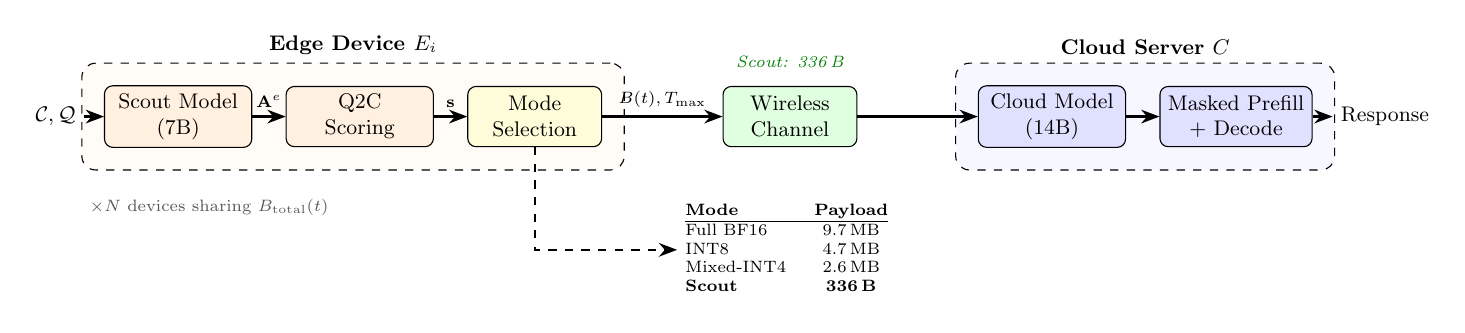
\begin{tikzpicture}[scale=0.85, every node/.style={transform shape},
    >=Stealth,
    box/.style={draw, rounded corners=3pt, minimum height=0.9cm, minimum width=1.6cm, font=\small, align=center, fill=#1},
    box/.default=blue!8,
    smallbox/.style={draw, rounded corners=2pt, minimum height=0.6cm, font=\scriptsize, align=center, fill=#1},
    smallbox/.default=gray!10,
    arr/.style={->, thick},
    darr/.style={->, thick, dashed},
    lbl/.style={font=\scriptsize, midway},
]

% --- Edge Device ---
\node[box=orange!12, minimum width=2.2cm] (edge_model) {Scout Model\\(7B)};
\node[box=orange!12, minimum width=2.2cm, right=0.5cm of edge_model] (q2c) {Q2C\\Scoring};
\node[box=yellow!15, minimum width=2.0cm, right=0.5cm of q2c] (mode_sel) {Mode\\Selection};

% Edge bounding box
\begin{scope}[on background layer]
\node[draw, dashed, rounded corners=5pt, fill=orange!3,
      fit=(edge_model)(q2c)(mode_sel),
      inner sep=8pt, label={[font=\small\bfseries]above:Edge Device $E_i$}] (edge_box) {};
\end{scope}

% --- Wireless Channel ---
\node[box=green!12, minimum width=2.0cm, right=1.8cm of mode_sel] (channel) {Wireless\\Channel};

% --- Cloud Server ---
\node[box=blue!12, minimum width=2.2cm, right=1.8cm of channel] (cloud_model) {Cloud Model\\(14B)};
\node[box=blue!12, minimum width=2.0cm, right=0.5cm of cloud_model] (decode) {Masked Prefill\\+ Decode};

% Cloud bounding box
\begin{scope}[on background layer]
\node[draw, dashed, rounded corners=5pt, fill=blue!3,
      fit=(cloud_model)(decode),
      inner sep=8pt, label={[font=\small\bfseries]above:Cloud Server $C$}] (cloud_box) {};
\end{scope}

% --- Arrows ---
\draw[arr] (edge_model) -- (q2c) node[lbl, above] {$\mathbf{A}^e$};
\draw[arr] (q2c) -- (mode_sel) node[lbl, above] {$\mathbf{s}$};

% Mode selection outputs
\draw[arr] (mode_sel) -- (channel) node[lbl, above, font=\scriptsize] {$B(t), T_{\max}$};

% Channel to cloud
\draw[arr] (channel) -- (cloud_model);

% Cloud internal
\draw[arr] (cloud_model) -- (decode);

% --- Mode labels below channel ---
\node[below=0.7cm of channel, font=\scriptsize, align=center] (modes) {
\begin{tabular}{@{}lc@{}}
\textbf{Mode} & \textbf{Payload} \\
\hline
Full BF16 & 9.7\,MB \\
INT8 & 4.7\,MB \\
Mixed-INT4 & 2.6\,MB \\
\textbf{Scout} & \textbf{336\,B} \\
\end{tabular}
};
\draw[darr] (mode_sel.south) |- (modes.west);

% --- Scout path highlight ---
\node[above=0.15cm of channel, font=\scriptsize\itshape, text=green!50!black] {Scout: 336\,B};

% --- Multi-agent annotation ---
\node[below=0.3cm of edge_box.south west, anchor=north west, font=\scriptsize, text=gray!70!black] (multi) {$\times N$ devices sharing $B_{\text{total}}(t)$};

% Response arrow
\node[right=0.3cm of decode, font=\small] (resp) {Response};
\draw[arr] (decode) -- (resp);

% Context input
\node[left=0.3cm of edge_model, font=\small] (ctx) {$\mathcal{C}, \mathcal{Q}$};
\draw[arr] (ctx) -- (edge_model);

\end{tikzpicture}
\caption{Scout system architecture. The edge device runs a lightweight scout model, computes Q2C attention scores, and selects an operating mode based on current bandwidth $B(t)$ and deadline $T_{\max}$. In scout mode, only 336~bytes of position indices traverse the wireless link (vs.\ 9.7\,MB for full KV-cache). The cloud re-prefills with its own model and applies the received position mask for decoding. $N$ edge devices share the base station bandwidth via model-aware allocation.}
\label{fig:system}
\end{figure*}


% ============================================================
% III. CROSS-MODEL ATTENTION ALIGNMENT
% ============================================================
\section{Cross-Model Attention Alignment}
\label{sec:attention}

\subsection{Why Attention Transfers}

Models in the same family share three critical properties: (1)~identical tokenization, ensuring the same input text maps to the same token positions; (2)~identical RoPE base frequency, ensuring consistent relative position encoding; and (3)~similar training data distributions, which shape attention patterns toward similar linguistic structures.

While KV-cache \emph{values} differ substantially between models (cosine similarity $\approx 0.22$), the \emph{attention patterns}---which positions receive high attention from query tokens---are more aligned, because they reflect the task structure rather than model-specific representations.

\textbf{Formal definition.}
Let $\mathbf{a}_i^{(s)}$ be the aggregated attention distribution of model~$s$ over context positions for query token~$i$.
We define the \emph{attention alignment} between two models $s_1, s_2$ at retention ratio $r$ as the expected Jaccard overlap:
\begin{equation}
    \mathcal{A}(s_1, s_2; r) = \mathbb{E}_{x}\left[\frac{|\text{top}_k(\mathbf{a}^{(s_1)}) \cap \text{top}_k(\mathbf{a}^{(s_2)})|}{|\text{top}_k(\mathbf{a}^{(s_1)}) \cup \text{top}_k(\mathbf{a}^{(s_2)})|}\right]
\end{equation}
where $k = \lfloor r \cdot n \rfloor$ and the expectation is over input samples $x$.
High alignment ($\mathcal{A} > 0.7$) indicates that the smaller model's selections are useful proxies for the larger model's preferences.

The key insight is that attention alignment is substantially higher than value similarity.
While KV-cache values encode model-specific representations (each model has different weight matrices), the \emph{positions} that receive high attention depend more on the task structure---which words contain the answer, which context is relevant to the query---than on the specific model producing the attention.

\subsection{Q2C Position Scoring}

We compute position importance using the \emph{Query-to-Context} (\QtoC) method.
For each context position~$j$, the score is the total attention weight received from all query positions at the last transformer layer:
\begin{equation}
    s_j = \sum_{h=1}^{H'} \sum_{i=n+1}^{n+m} \bA^{(L,h)}_{i,j}
    \label{eq:q2c_score}
\end{equation}
where $L$ is the last layer, $H'$ is the number of attention heads at layer $L$, $n$ is the context length, and $m$ is the query length.
This aggregates all attention that query tokens pay to each context position, directly measuring task relevance.\footnote{Ablation confirms that averaging across all layers yields equivalent rankings: Pearson $r > 0.99$ for all three tested models (Section~\ref{sec:ablation}).}

Given a retention ratio $r$, we select the top-$\lfloor r \cdot n \rfloor$ context positions by \QtoC score.
Unselected positions are masked by setting their attention weights to $-\infty$ during decoding, preserving the RoPE positional encoding of retained positions.

\subsection{Same-Family Alignment}

Table~\ref{tab:scout_n200} presents position overlap and task quality results across three model pairs in the Qwen2.5 family ($n = 200$ SQuAD~v2 samples, 95\% CIs).
Fig.~\ref{fig:scout_overlap} visualizes the overlap and F1 comparison.

\begin{table*}[t]
\centering
\caption{Scout model validation within the Qwen2.5 family ($n = 200$, SQuAD~v2, normalized token-F1, $\pm$95\% CI). Boldface = scout F1 $\geq$ cloud's own F1. $p$-values from paired $t$-test with Bonferroni correction (9~comparisons, $\alpha = 0.0056$).}
\label{tab:scout_n200}
\small
\begin{tabular}{@{}llcccccc@{}}
\toprule
\textbf{Pair} & \textbf{Ret.} & \textbf{Overlap (\%)} & \textbf{Cloud Own F1} & \textbf{Scout F1} & \textbf{Gap} & \textbf{$p$-value} & \textbf{Sig.?} \\
\midrule
\multirow{3}{*}{3B$\to$7B}
  & 75\% & 81.6 & 0.615 $\pm$ 0.057 & 0.525 $\pm$ 0.059 & $-$0.091 & 0.0016 & Yes \\
  & 50\% & 63.8 & 0.543 $\pm$ 0.058 & 0.356 $\pm$ 0.055 & $-$0.187 & $<$0.001 & Yes \\
  & 25\% & 45.0 & 0.339 $\pm$ 0.055 & 0.222 $\pm$ 0.049 & $-$0.117 & $<$0.001 & Yes \\
\midrule
\multirow{3}{*}{3B$\to$14B}
  & 75\% & 83.2 & 0.664 $\pm$ 0.054 & 0.542 $\pm$ 0.059 & $-$0.122 & $<$0.001 & Yes \\
  & 50\% & 70.4 & 0.499 $\pm$ 0.059 & 0.405 $\pm$ 0.057 & $-$0.094 & 0.004 & Yes \\
  & 25\% & 58.7 & 0.322 $\pm$ 0.056 & 0.246 $\pm$ 0.050 & $-$0.076 & 0.012 & No \\
\midrule
\multirow{3}{*}{7B$\to$14B}
  & 75\% & 83.7 & 0.664 $\pm$ 0.054 & \textbf{0.661} $\pm$ 0.055 & $-$0.004 & 0.883 & No \\
  & 50\% & 69.5 & 0.499 $\pm$ 0.059 & \textbf{0.546} $\pm$ 0.058 & $+$0.047 & 0.110 & No \\
  & 25\% & 54.8 & 0.322 $\pm$ 0.056 & \textbf{0.381} $\pm$ 0.058 & $+$0.059 & 0.039 & No \\
\bottomrule
\end{tabular}
\end{table*}

\begin{figure}[t]
    \centering
    \includegraphics[width=\columnwidth]{fig2_scout_overlap_f1.pdf}
    \caption{Cross-model scout results ($n = 200$). (a)~Position overlap between edge and cloud models' Q2C selections. (b)~F1 comparison: faded bars = cloud's own selection; solid bars = scout selection applied to cloud. The 7B$\to$14B pair (green) shows scout matching or slightly exceeding cloud own at all retentions.}
    \label{fig:scout_overlap}
\end{figure}

Table~\ref{tab:cross_arch_overlap} extends this analysis across three architectures.

\begin{table}[t]
\centering
\caption{Cross-architecture scout overlap ($n = 200$, SQuAD~v2, 75\% retention). All families show 84--92\% overlap; scout F1 is statistically indistinguishable from cloud's own selection ($p > 0.05$).}
\label{tab:cross_arch_overlap}
\footnotesize
\begin{tabular}{@{}llcccc@{}}
\toprule
\textbf{Family} & \textbf{Pair} & \textbf{Overlap} & \textbf{Scout F1} & \textbf{Gap} & $p$ \\
\midrule
Qwen 2.5  & 7B$\to$14B  & 83.7\% & 0.661 & $-$0.004 & 0.883 \\
Llama 3   & 3B$\to$8B   & 91.8\% & 0.224 & $-$0.032 & 0.060 \\
Gemma 2   & 2B$\to$9B   & 86.1\% & 0.397 & $+$0.022 & 0.359 \\
\midrule
\multicolumn{2}{@{}l}{\textit{Cross-family:}} \\
Qwen$\to$Mis. & 7B$\to$7B & 73.4\% & 0.167 & $+$0.045 & 0.013 \\
\bottomrule
\end{tabular}
\end{table}

\textbf{Finding 1: 84--92\% overlap at 75\% retention across architectures.}
Same-family overlap is consistently high: 83.7\% (Qwen), 91.8\% (Llama), and 86.1\% (Gemma).
This is substantially above the cross-family baseline (73.4\% for Qwen$\to$Mistral), confirming that shared tokenizer and training distribution---not just shared attention mechanism---drive alignment.
Overlap decreases to 64--86\% at 50\% and 45--81\% at 25\%, following the expected set-intersection scaling.

\textbf{Finding 2: Scout matches cloud's own selection across all three families.}
No same-family pair shows a statistically significant quality gap at 75\% retention: Qwen 7B$\to$14B ($p = 0.883$), Llama 3B$\to$8B ($p = 0.060$), Gemma 2B$\to$9B ($p = 0.359$).
Gemma's scout shows a positive gap ($+0.022$), and Llama's borderline result ($-0.032$, $p = 0.06$) does not reach significance.
This confirms that scout selection is \emph{statistically indistinguishable} from the cloud model's own selection at the primary operating point---a result that generalizes across architectures with different attention mechanisms (GQA with 4--8 KV heads), vocabulary sizes (128K--256K), and training corpora.

\textbf{Finding 3: Within-Qwen, 3B scout incurs meaningful quality loss.}
The Qwen 3B$\to$7B and 3B$\to$14B pairs show significant quality gaps at 75\% and 50\% retention, indicating that the 3B model's attention is insufficiently focused to substitute for larger models' selections.
This suggests a minimum scout model capability threshold.
Notably, Llama's 3B$\to$8B and Gemma's 2B$\to$9B pairs---despite using similarly small edge models---do not show significant degradation, suggesting this threshold is family-specific rather than universal.

\textbf{Finding 4: Extreme bandwidth savings.}
Scout reduces the transmission payload from 9.7--100.7\,MB (full KV) to 336~bytes (position indices for $\sim$128 positions at 75\% retention of a $\sim$170-token context)---a 28{,}800--300{,}000$\times$ reduction.
At 100\,Mbps, this reduces TX time from 775--8{,}056\,ms to 0.03\,ms.
Table~\ref{tab:compression_comparison} puts this in perspective against prior work.

\begin{table}[t]
\centering
\caption{Compression ratio comparison with prior work.}
\label{tab:compression_comparison}
\small
\begin{tabular}{@{}lccl@{}}
\toprule
\textbf{Method} & \textbf{Ratio} & \textbf{Transmits} & \textbf{Constraint} \\
\midrule
CacheGen~\cite{cachegen}  & 3.5$\times$  & KV data  & Same model \\
INT8 quantization          & 2$\times$    & KV data  & Same model \\
INT4 quantization          & 4$\times$    & KV data  & Same model \\
SnapKV (50\% ret.)         & 2$\times$    & KV data  & Same model \\
Scout (this work)          & \textbf{28,800}$\times$ & Indices & Same family \\
\bottomrule
\end{tabular}
\end{table}

\subsection{Cross-Family Alignment}

We test whether attention alignment extends beyond family boundaries by pairing Qwen2.5-7B (edge) with Mistral-7B-v0.3 (cloud).
Table~\ref{tab:cross_family} presents the results ($n = 200$).

\begin{table}[t]
\centering
\caption{Cross-family scout: Qwen-7B $\to$ Mistral-7B ($n = 200$, SQuAD~v2). Note: Mistral-7B baseline F1 = 0.258 on this task.}
\label{tab:cross_family}
\small
\begin{tabular}{@{}lcccc@{}}
\toprule
\textbf{Ret.} & \textbf{Overlap} & \textbf{Cloud Own} & \textbf{Scout F1} & \textbf{$p$-value} \\
\midrule
75\% & 73.4\% & 0.122 & 0.167 & 0.013 \\
50\% & 58.6\% & 0.082 & 0.102 & 0.054 \\
25\% & 41.4\% & 0.063 & 0.059 & 0.360 \\
\bottomrule
\end{tabular}
\end{table}

Cross-family overlap is lower than same-family (73\% vs.\ 84\% at 75\% retention), reflecting different architectural choices and training procedures.
Notably, the Qwen-7B scout \emph{improves} Mistral's quality at 75\% retention ($p = 0.013$), suggesting that Qwen's more focused attention can benefit Mistral even without shared training.
However, Mistral-7B's low baseline F1 (0.258 on SQuAD~v2) limits the practical significance of these results.

\subsection{Attention Entropy Analysis}

We analyze the \QtoC score distribution entropy as a measure of attention concentration.
Higher entropy indicates more diffuse attention across positions; lower entropy indicates focused attention on fewer positions.

\begin{table}[t]
\centering
\caption{Attention entropy of Q2C score distributions ($n = 200$). Lower entropy = more focused attention.}
\label{tab:entropy}
\small
\begin{tabular}{@{}lcccc@{}}
\toprule
\textbf{Model} & \textbf{Overall} & \textbf{Last Layer} & \textbf{Q2C Dist.} \\
\midrule
Qwen2.5-3B  & 2.61 $\pm$ 0.03 & 3.31 $\pm$ 0.04 & 4.21 $\pm$ 0.12 \\
Qwen2.5-7B  & 2.56 $\pm$ 0.03 & 3.01 $\pm$ 0.05 & 5.49 $\pm$ 0.07 \\
Qwen2.5-14B & 2.13 $\pm$ 0.02 & 3.67 $\pm$ 0.05 & 4.65 $\pm$ 0.07 \\
\bottomrule
\end{tabular}
\end{table}

The relationship between model size and attention entropy is non-monotonic: 3B has the lowest \QtoC distribution entropy (4.21), 14B is intermediate (4.65), and 7B has the highest (5.49).
This has practical implications for the scout protocol:

\textbf{The attention focusing hypothesis.}
The 3B model's low entropy indicates highly concentrated attention on a small set of positions.
This extreme concentration may cause it to miss positions that larger models identify through broader attention patterns, explaining the quality gap in 3B$\to$7B and 3B$\to$14B scouting.
In contrast, the 7B model's broader attention (higher entropy) captures a more complete set of task-relevant positions, producing selections that align well with the 14B model.

\textbf{Why 7B matches 14B.}
The 14B model has lower \QtoC entropy than the 7B (4.65 vs.\ 5.49), meaning it focuses \emph{more} than the 7B.
When the 7B scout's broader selection is applied as a mask to the 14B, the 14B's own focused attention within that mask naturally concentrates on the most relevant positions.
The 7B's selection acts as a \emph{superset} filter: it contains most positions the 14B would select (83.7\% overlap) plus additional positions that provide a safety margin.
This explains why the scout quality matches rather than degrades: the 14B model effectively ``ignores'' the extra positions through its own attention mechanism.

\textbf{Implications for scout model selection.}
Our findings suggest that the ideal scout model should have sufficiently broad attention to capture all positions the cloud model considers important, while being compact enough to run at the edge.
Within the Qwen2.5 family, the 7B model achieves this balance for the 14B cloud.
Cross-architecture experiments (Section~\ref{sec:experiments}) confirm this pattern generalizes: Llama~3B achieves 91.8\% overlap with Llama~8B, and Gemma~2B achieves 86.1\% with Gemma~9B.


% ============================================================
% IV. SCOUT PROTOCOL DESIGN
% ============================================================
\section{Scout Protocol Design}
\label{sec:protocol}

\subsection{Protocol Description}

Algorithm~\ref{alg:scout} describes the Scout protocol for a single inference request.

\begin{algorithm}[t]
\caption{Scout Protocol}
\label{alg:scout}
\SetAlgoLined
\KwIn{Context $\mathcal{C}$, query $\mathcal{Q}$, bandwidth $B(t)$, deadline $T_{\max}$}
\KwOut{Generated response}

\tcp{Edge device}
$\mathcal{K}^e, \mathcal{V}^e, \mathbf{A}^e \leftarrow \text{Prefill}_{M^{\text{edge}}}(\mathcal{C}, \mathcal{Q})$\;
$\mathbf{s} \leftarrow \text{Q2C}(\mathbf{A}^e)$ \tcp*{Compute attention scores}

\tcp{Mode selection based on bandwidth}
$\text{mode} \leftarrow \text{SelectMode}(B(t), T_{\max}, |\mathcal{K}^e|)$\;

\Switch{mode}{
    \Case{FULL\_KV}{
        Transmit $\mathcal{K}^e, \mathcal{V}^e$ in BF16\;
        Cloud: decode with received KV\;
    }
    \Case{QUANT\_KV}{
        $\hat{\mathcal{K}}, \hat{\mathcal{V}} \leftarrow \text{Quantize}(\mathcal{K}^e, \mathcal{V}^e, b)$\;
        Transmit $\hat{\mathcal{K}}, \hat{\mathcal{V}}$\;
        Cloud: dequantize and decode\;
    }
    \Case{SCOUT}{
        $\mathcal{S} \leftarrow \text{TopK}(\mathbf{s}, \lfloor r \cdot n \rfloor)$ \tcp*{Position indices}
        Transmit $\mathcal{S}$ (compact index list)\;
        Cloud: $\mathcal{K}^c, \mathcal{V}^c \leftarrow \text{Prefill}_{M^{\text{cloud}}}(\mathcal{C}, \mathcal{Q})$\;
        Cloud: mask to $\mathcal{S}$, decode\;
    }
}
\Return{response}
\end{algorithm}

In scout mode, the cloud \emph{re-executes} the prefill phase with its own model to generate its own KV-cache, then applies the edge's position mask via attention masking (setting unselected positions to $-\infty$ in the attention score matrix).
This preserves RoPE positional encoding correctness, unlike physical KV removal which breaks position continuity.

\textbf{Why not simply retransmit the original text?}
A natural question is why not send the raw prompt to the cloud, bypassing KV-cache transfer entirely.
In fact, scout mode approximates this---the cloud re-prefills from the original tokens.
The key added value is the position mask: it enables the cloud to apply KV-cache eviction \emph{without running its own selection pass}, reducing decode-time memory and attention cost from $O(n)$ to $O(rn)$ per generated token.
This benefit grows with context length: at 32K tokens, attending to 75\% saves 8K positions per decode step.
Moreover, the position mask enables the \emph{adaptive protocol}: the same edge prefill simultaneously produces (1)~the compressed KV-cache for transmission when bandwidth permits, and (2)~the position indices as a zero-bandwidth fallback.
Without the edge model's analysis, the cloud would need to either receive the full KV-cache or perform its own full prefill with no eviction guidance---forgoing the bandwidth-quality adaptation that defines our protocol.

\subsection{Mode Selection Policy}

The mode selection function maps current bandwidth and deadline constraints to the highest-quality operating mode that meets the latency requirement:
\begin{equation}
    \text{mode}^* = \arg\max_{m \in \mathcal{M}} Q(m) \quad \text{s.t.} \quad T(m, B(t)) \leq T_{\max}
    \label{eq:mode_select}
\end{equation}
where $\mathcal{M}$ is the set of operating modes, $Q(m)$ is the pre-calibrated quality for mode~$m$, and $T(m, B)$ is the end-to-end latency.
Since $|\mathcal{M}| \leq 5$, this is solved by enumeration in constant time.

\subsection{Protocol Overhead}

The Scout protocol's control plane adds minimal overhead:
\begin{itemize}
    \item \textbf{Handshake}: Model family identification, capability exchange ($<$100 bytes).
    \item \textbf{Mode advertisement}: Current bandwidth estimate + selected mode ($<$50 bytes).
    \item \textbf{Position indices}: $k \times 2$ bytes for $k$ selected positions (16-bit indices suffice for contexts up to 65{,}536 tokens).
\end{itemize}
Total control overhead is $<$1\,KB, negligible compared to even the smallest KV payload.

\subsection{Latency Breakdown}

Table~\ref{tab:scout_latency} breaks down the end-to-end latency for scout mode compared to KV-cache transmission modes.

\begin{table}[t]
\centering
\caption{End-to-end latency comparison for 7B$\to$14B (ms, 100\,Mbps).}
\label{tab:scout_latency}
\small
\begin{tabular}{@{}lccccc@{}}
\toprule
\textbf{Mode} & \textbf{E-Prefill} & \textbf{Compress} & \textbf{TX} & \textbf{C-Prefill} & \textbf{Total} \\
\midrule
Full BF16 & 18 & --- & 780 & --- & 798 \\
INT8      & 18 & 3   & 390 & --- & 411 \\
Scout     & 18 & 0   & 0.03 & 57 & 75 \\
\bottomrule
\end{tabular}
\end{table}

Scout mode total latency (75\,ms) is 10.6$\times$ faster than full BF16 (798\,ms) and 5.5$\times$ faster than INT8 (411\,ms).
The dominant cost shifts from network transmission (780\,ms for BF16) to cloud prefill computation (57\,ms for scout).
Scout thus trades cloud-side compute (57\,ms prefill) for bandwidth savings (9.7\,MB $\to$ 336\,B); this tradeoff favors scout at bandwidths below $\sim$200\,Mbps, where transmission dominates total latency.
When the cloud would have performed prefill anyway (\eg, for prompt validation or multi-turn context extension), the marginal cost of scout is near zero.

\subsection{Hybrid Mode}

We investigate a hybrid mode that transmits both position indices and partial KV-cache data for a subset of layers, potentially providing higher quality than pure scout while remaining more bandwidth-efficient than full KV transfer.

Using the 7B$\to$14B pair ($n = 200$), we test transmitting the scout's position indices plus 1--2 layers of the 7B model's KV-cache.
Results show that hybrid modes produce \emph{identical} F1 to pure scout (0.661 vs.\ 0.661 at 75\%), because the cloud model generates its own KV-cache during prefill and the cross-model KV values are incompatible (cosine similarity $\approx 0.22$).
The additional KV data from the edge model does not improve quality but increases payload from 336~bytes to 247\,KB (1~layer) or 495\,KB (2~layers).
Therefore, pure scout mode dominates hybrid mode for same-family model pairs.

\subsection{Multi-Turn Extension}

In multi-turn dialogue, the scout protocol extends naturally.
For each new turn, the edge model processes the incremental context and generates updated \QtoC scores.
Only the \emph{delta} position set (new positions to add, old positions to remove) needs transmission, reducing per-turn payload further.
The cloud maintains its own KV-cache across turns and applies the updated mask.
This multi-turn extension preserves the sub-KB payload advantage while supporting conversational applications.


% ============================================================
% V. KV-CACHE COMPRESSION OPERATING POINTS
% ============================================================
\section{KV-Cache Compression Operating Points}
\label{sec:compression}

When bandwidth permits, transmitting compressed KV-cache data can achieve higher quality than scout mode.
This section characterizes the compression landscape to inform protocol mode selection.
Fig.~\ref{fig:operating_points} shows the quality-bandwidth Pareto frontier.

\begin{figure}[t]
    \centering
    \includegraphics[width=\columnwidth]{fig9_operating_points.pdf}
    \caption{Quality-bandwidth operating points for Qwen-7B ($n = 200$). Each point represents a compression mode. Scout achieves near-100\% quality at near-zero bandwidth. The dashed line marks the full-KV baseline.}
    \label{fig:operating_points}
\end{figure}

\subsection{Token Selection Methods}

We compare three selection methods: \QtoC (last-layer query-to-context attention), SnapKV~\cite{snapkv} (observation-window attention), and H2O~\cite{h2o} (cumulative attention eviction).
Table~\ref{tab:selection_unified} presents results on Qwen-7B with $n = 200$ samples.

\begin{table}[t]
\centering
\caption{Selection method comparison (Qwen-7B, SQuAD~v2, $n = 200$, normalized token-F1, $\pm$95\% CI). $p$-values from paired $t$-test.}
\label{tab:selection_unified}
\small
\begin{tabular}{@{}lccc@{}}
\toprule
\textbf{Retention} & \textbf{\QtoC} & \textbf{SnapKV} & \textbf{H2O} \\
\midrule
75\% & 0.608 $\pm$ 0.059 & 0.608 $\pm$ 0.059 & 0.558 $\pm$ 0.059 \\
50\% & 0.541 $\pm$ 0.058 & 0.544 $\pm$ 0.058 & 0.380 $\pm$ 0.059 \\
25\% & 0.368 $\pm$ 0.057 & 0.366 $\pm$ 0.057 & 0.246 $\pm$ 0.049 \\
\midrule
\multicolumn{4}{@{}l}{\textit{Pairwise $p$-values (paired $t$-test):}} \\
\multicolumn{4}{@{}l}{Q2C vs.\ SnapKV: $p = 0.32$--$0.75$ (NS at all retentions)} \\
\multicolumn{4}{@{}l}{Q2C vs.\ H2O: $p = 0.056$ (75\%); $p < 10^{-5}$ (50\%);} \\
\multicolumn{4}{@{}l}{\quad $p = 2.65 \times 10^{-5}$ (25\%)} \\
\bottomrule
\end{tabular}
\end{table}

\QtoC and SnapKV produce statistically indistinguishable results at all retention levels ($p = 0.32$--$0.75$).\footnote{Per-sample analysis reveals that \QtoC and SnapKV select identical position sets for 199 of 200 samples at 75\% retention. Despite different scoring mechanisms (last-layer attention sum vs.\ observation-window voting), both converge to the same top-$k$ positions on this dataset, explaining the identical $p$-values at 75\% and 50\% retention.}
Both significantly outperform H2O at 50\% and 25\% retention ($p < 10^{-5}$ and $p = 2.65 \times 10^{-5}$, respectively).
At 75\% retention---the primary operating point---Q2C and H2O show marginal separation ($p = 0.056$); the gap widens sharply at lower retentions because H2O's attention-sink bias~\cite{streamingllm} becomes more severe with aggressive token removal.
The practical advantage of \QtoC is its simplicity: it requires a single attention extraction at the last layer, whereas SnapKV needs an observation window.

\subsection{Quantization Characterization}

Table~\ref{tab:quantization} presents quantization results across 5~models ($n = 200$, SQuAD~v2).

\begin{table}[t]
\centering
\caption{Quantization quality as F1 and \% of BF16 baseline ($n = 200$, SQuAD~v2). Sensitive layers identified by per-layer INT4 probing.}
\label{tab:quantization}
\small
\begin{tabular}{@{}lcccc@{}}
\toprule
\textbf{Model} & \textbf{INT8} & \textbf{INT4} & \textbf{Mixed} & \textbf{Sensitive} \\
\midrule
Qwen-7B    & 99.4\% & 68.7\% & 93.6\% & L0 \\
Qwen-14B   & 100\%  & 95.5\% & 95.6\% & None \\
Yi-6B      & 99.5\% & 100\%  & 100\%  & None \\
Mistral-7B & 99.8\% & 96\%   & 94\%   & None \\
Qwen-3B    & 100\%  & 96\%   & ---    & L0 (weak) \\
\bottomrule
\end{tabular}
\end{table}

\textbf{INT8 is universally lossless.}
Across all 5~models, INT8 quantization preserves $\geq$99.4\% of baseline quality (Wilcoxon $p > 0.7$ for all models).

\textbf{INT4 fragility is model-specific.}
INT4 quality ranges from 68.7\% (Qwen-7B) to 100\% (Yi-6B).
Critically, Yi-6B and Qwen-7B share identical GQA configurations (4~KV heads, 128 head dimension) but exhibit opposite INT4 behavior, \emph{refuting} the hypothesis that INT4 sensitivity is determined by architecture.
This is an emergent property of the training procedure.

\textbf{Mixed-precision recovers concentrated damage.}
For Qwen-7B, where INT4 damage localizes to Layer~0, keeping only this layer at FP16 (rest INT4) recovers quality from 68.7\% to 93.6\% at minimal bandwidth cost ($\bar{b} = 4.43$ bits, 27.7\% of BF16).
The discovery process is simple: run per-layer INT4 sensitivity analysis (one-time cost per model), identify layers where individual INT4 quantization causes $>$3\% degradation, and protect them at FP16.
Concurrent work KVTuner~\cite{kvtuner} addresses this problem through learned bit-width allocation; our focus is on cross-architecture characterization for protocol design rather than optimization.

\textbf{Two damage patterns.}
When INT4 degrades quality by ${>}5\%$, we observe two patterns:
\begin{itemize}
    \item \emph{Concentrated}: Damage localizes to one layer (Layer~0 for Qwen-7B/3B). Mixed-precision achieves full recovery.
    \item \emph{Distributed}: Damage spreads across many layers. Mixed-precision provides no benefit; use INT8 instead.
\end{itemize}

\subsection{Task-Dependent Quantization Sensitivity}

INT4 sensitivity varies not only across models but across tasks.
For Qwen-7B (the most INT4-fragile model), extractive QA (SQuAD) degrades to 77\% while multiple-choice (MMLU) retains 100\% quality at INT4.
Tasks requiring precise token localization are most sensitive, while reasoning tasks that can tolerate approximate representations are robust.
This task dependency further motivates the adaptive protocol: the same model may safely use INT4 for some task types but require INT8 or mixed-precision for others.

\subsection{Perplexity Validation}

To complement task-specific F1 evaluation, we measure perplexity on WikiText-2 with KV-cache quantization (100 segments).
Table~\ref{tab:perplexity} confirms the task-based findings.

\begin{table}[t]
\centering
\caption{WikiText-2 perplexity with KV-cache quantization (100 segments, lower is better).}
\label{tab:perplexity}
\small
\begin{tabular}{@{}lcccc@{}}
\toprule
\textbf{Model} & \textbf{BF16} & \textbf{INT8} & \textbf{INT4} & \textbf{Mixed} \\
\midrule
Qwen-7B    & 8.63  & 8.85  & \textbf{80.27} & 8.97  \\
Qwen-14B   & 5.73  & 5.73  & 5.87  & 5.83  \\
Mistral-7B & 6.49  & 6.49  & 6.51  & 6.51  \\
\bottomrule
\end{tabular}
\end{table}

Qwen-7B's INT4 perplexity (80.27) is catastrophic---9.3$\times$ over BF16 (8.63)---while Qwen-14B and Mistral-7B show $<$3\% increase, confirming the model-specificity of INT4 fragility (Fig.~\ref{fig:perplexity}).
INT8 is lossless for all three models (PPL increase $<$0.3), independently validating the task-based F1 findings.

\begin{figure}[t]
    \centering
    \includegraphics[width=\columnwidth]{fig4_perplexity.pdf}
    \caption{WikiText-2 perplexity with KV-cache quantization. Qwen-7B's INT4 perplexity (80.27) is catastrophic, while Qwen-14B and Mistral-7B are robust. INT8 is universally lossless.}
    \label{fig:perplexity}
\end{figure}

\subsection{Delta Encoding Counter-Finding}

Delta encoding---the core technique in CacheGen~\cite{cachegen}---reduces key variance by up to 735$\times$ via anchor-based differencing.
However, we find it \emph{degrades} task quality: anchor INT4 achieves only 66.9\% of BF16 vs.\ 72.5\% for direct INT4 ($n = 50$, Qwen-7B, SQuAD~v2).
The root cause is that delta values distribute more uniformly across the quantization range, increasing per-element error; entropy analysis confirms delta-encoded INT4 requires 7.94 bits/element vs.\ 6.13 for direct INT4.
This counter-finding motivates our choice of direct quantization over delta encoding in the protocol's compression modes.

\subsection{Latency Analysis}

Transmission dominates end-to-end latency: at 100\,Mbps, Qwen-7B BF16 KV transfer takes 780\,ms (97\% of total) with quantization overhead of only 2.7--3.4\,ms.
INT8 halves transmission time (2.7\,s $\to$ 1.3\,s for Qwen-14B) with 4.8\,ms overhead, yielding 44\% net latency reduction.
At 10\,Mbps (typical edge uplink), uncompressed Qwen-14B requires 26.8\,s; INT4 reduces this to 6.7\,s.


% ============================================================
% VI. ADAPTIVE TRANSPORT PROTOCOL
% ============================================================
\section{Adaptive Transport Protocol}
\label{sec:transport}

\subsection{Mode Selection with Real 5G Traces}

We evaluate the adaptive protocol using real 5G network traces from the Lumos5G dataset~\cite{lumos5g}, covering four scenarios with mean throughput ranging from 50\,Mbps (vehicular) to 173\,Mbps (urban mmWave), with high variability (std dev 29--134\,Mbps).

The protocol uses Table~\ref{tab:operating_points} as a lookup table to select the highest-quality mode whose transmission time fits within the deadline at the current bandwidth.
For each operating mode~$m$ with payload size $S(m)$ bytes, the transmission time at bandwidth $B$ is:
\begin{equation}
    T_{\text{TX}}(m, B) = \frac{8 \cdot S(m)}{B}
    \label{eq:tx_time}
\end{equation}
The total latency includes prefill, compression, transmission, and decode:
\begin{equation}
    T(m, B) = T_{\text{prefill}} + T_{\text{compress}}(m) + T_{\text{TX}}(m, B) + T_{\text{decode}}
\end{equation}

The protocol selects the mode that maximizes quality subject to the deadline:
\begin{equation}
    m^* = \arg\max_{m \in \mathcal{M}} Q(m) \quad \text{s.t.} \quad T(m, B(t)) \leq T_{\max}
\end{equation}

When no KV-based mode meets the deadline, the protocol falls back to scout mode, which meets any realistic deadline due to its $<$1\,KB payload.
This provides a graceful degradation guarantee: the system always produces a response, with quality determined by the available bandwidth.

\subsection{Bandwidth Estimation}

In practice, $B(t)$ is estimated using exponentially weighted moving average (EWMA) of recent throughput measurements:
\begin{equation}
    \hat{B}(t) = \alpha \cdot B_{\text{measured}}(t) + (1 - \alpha) \cdot \hat{B}(t-1)
\end{equation}
with $\alpha = 0.3$ providing responsiveness while avoiding oscillation.
The protocol uses a conservative estimate ($\hat{B} \times 0.8$) for mode selection to account for estimation error.
This approach mirrors adaptive bitrate (ABR) algorithms used in video streaming~\cite{abr}, adapted to the discrete nature of KV-cache compression modes.

\subsection{Multi-Agent Bandwidth Allocation}

When $N$ edge devices share a base station with total bandwidth $B_{\text{total}}$, the allocation problem becomes:
\begin{equation}
    \max_{\{B_i\}} \sum_{i=1}^{N} Q_i^*(B_i)
    \quad \text{s.t.} \quad \sum_{i=1}^{N} B_i \leq B_{\text{total}}, \quad T_i(B_i) \leq T_{\max}
    \label{eq:multiagent}
\end{equation}
where $Q_i^*(B_i) = \max_{m \in \mathcal{M}_i} \{Q_i(m) : T_i(m, B_i) \leq T_{\max}\}$.

We compare three allocation strategies:

\textbf{Equal allocation}: $B_i = B_{\text{total}} / N$ for all $i$.

\textbf{Model-aware proportional}: $B_i = B_{\text{total}} \times S_i / \sum_j S_j$ where $S_i$ is the KV-cache size of model~$M_i$, ensuring similar transmission times.

\textbf{Quality-maximizing}: Greedy assignment of bandwidth to the device with the largest quality gain from the next increment.

When bandwidth is insufficient for KV-cache transfer within the deadline, devices fall back to scout mode (transmit position indices only) or local inference (edge model generates response alone).
Both fallback modes provide guaranteed deadline compliance, ensuring the system never fails silently.

\subsection{Deadline-Aware Fallback Hierarchy}

The complete fallback hierarchy, in decreasing quality and bandwidth order:
\begin{enumerate}
    \item Full BF16 KV-cache transfer (quality: 100\%, highest bandwidth)
    \item INT8 quantized KV-cache (quality: 99.4\%, 50\% bandwidth)
    \item Mixed-INT4 quantized KV-cache (quality: 93.6\%, 27.7\% bandwidth)
    \item INT4 quantized KV-cache (quality: 68.7\%, 25\% bandwidth)
    \item Scout mode with position indices (quality: $\sim$100\% for 7B$\to$14B, $<$1\,KB)
    \item Local edge inference (quality: 60--75\% of cloud, zero bandwidth)
\end{enumerate}

The protocol engine traverses this hierarchy from top to bottom, selecting the first mode whose latency fits within the deadline.
This ensures maximum quality for the available bandwidth while guaranteeing response delivery.

\subsection{Comparison with CacheGen}

Compared to CacheGen~\cite{cachegen}---the most directly comparable system---Scout differs in three fundamental ways: (1)~Scout transmits position indices (28,800$\times$ compression) rather than compressed KV data (3.5$\times$); (2)~Scout adapts across 5~modes in real time, whereas CacheGen is static; and (3)~Scout supports cross-model transfer, while CacheGen requires identical sender and receiver models.
Our delta encoding counter-finding (Section~\ref{sec:compression}) provides additional evidence that CacheGen's core technique degrades quality when combined with quantization.


% ============================================================
% VII. EXPERIMENTAL EVALUATION
% ============================================================
\section{Experimental Evaluation}
\label{sec:experiments}

\subsection{Setup}

\textbf{Models.}
We evaluate 9~models from 5~families: Qwen2.5-3B/7B/14B, Llama-3.2-3B and 3.1-8B, Gemma-2-2B and 2-9B, Mistral-7B-v0.3, and Yi-1.5-6B (Table~\ref{tab:models}).
All models use BFloat16 precision with eager attention implementation to extract per-layer attention weights.

\textbf{Tasks.}
Primary evaluation uses SQuAD~v2~\cite{squad} (extractive QA, token-F1); secondary evaluation uses HotpotQA~\cite{hotpotqa} (multi-hop reasoning).
Context lengths range from 100--500 tokens (standard) and up to 2048 tokens (long-context experiments).

\textbf{Sample sizes and statistics.}
All experiments use $n = 200$ samples unless otherwise noted.
We report 95\% confidence intervals from paired $t$-tests.
Where multiple comparisons are made, we apply Bonferroni correction and note the adjusted significance threshold.

\textbf{Hardware.}
GPU experiments ran on NVIDIA A100 SXM4 (40\,GB and 80\,GB) and RTX 3090 GPUs via vast.ai.
Protocol simulations run on CPU.

\subsection{Scout Validation ($n = 200$)}

The scout validation results in Table~\ref{tab:scout_n200} demonstrate three key findings:

(1)~\emph{7B scout matches 14B's own selection at 75\% retention.}
The gap is $-0.004$ ($p = 0.883$), statistically indistinguishable.
At lower retentions, positive trends emerge ($+0.047$ at 50\%, $+0.059$ at 25\%) but do not reach significance after Bonferroni correction.

(2)~\emph{3B scout is insufficient for production use.}
At 75\% retention, 3B$\to$7B loses 0.091 ($p = 0.002$) and 3B$\to$14B loses 0.122 ($p < 0.001$), both significant.

(3)~\emph{Overlap generalizes across architectures.}
Same-family overlap at 75\% is consistent within Qwen (82--84\%) and extends to Llama~3 (91.8\%) and Gemma~2 (86.1\%), as shown in Table~\ref{tab:cross_arch_overlap}.

\subsection{Multitask Scout Validation}

Table~\ref{tab:multitask} extends scout validation to HotpotQA ($n = 100$ per task, 7B$\to$14B pair).

\begin{table}[t]
\centering
\caption{Multitask scout validation (7B$\to$14B, $n = 100$ per task, $\pm$95\% CI).}
\label{tab:multitask}
\small
\begin{tabular}{@{}llcccc@{}}
\toprule
\textbf{Task} & \textbf{Ret.} & \textbf{Overlap} & \textbf{Scout F1} & \textbf{Gap} & $p$ \\
\midrule
\multirow{3}{*}{SQuAD}
  & 75\% & 84.0\% & 0.691 $\pm$ 0.076 & $+$0.007 & 0.839 \\
  & 50\% & 69.7\% & 0.560 $\pm$ 0.082 & $+$0.088 & \textbf{0.026} \\
  & 25\% & 54.1\% & 0.367 $\pm$ 0.081 & $+$0.085 & \textbf{0.039} \\
\midrule
\multirow{3}{*}{HotpotQA}
  & 75\% & 84.7\% & 0.579 $\pm$ 0.088 & $-$0.014 & 0.626 \\
  & 50\% & 72.7\% & 0.510 $\pm$ 0.088 & $-$0.010 & 0.772 \\
  & 25\% & 58.9\% & 0.560 $\pm$ 0.087 & $+$0.009 & 0.847 \\
\bottomrule
\end{tabular}
\end{table}

On SQuAD, the scout shows significant positive effects at 50\% ($+0.088$, $p = 0.026$) and 25\% retention ($+0.085$, $p = 0.039$).
On HotpotQA, the scout is neutral (gaps $<$0.015, $p > 0.6$)---the multi-hop reasoning task's quality is less sensitive to position selection, as relevant information is more distributed.

\subsection{Long Context Overlap Stability}

Table~\ref{tab:long_ctx} shows that position overlap remains stable as context length increases from 1024 to 2048 tokens (7B$\to$14B pair, $n = 100$ per length).

\begin{table}[t]
\centering
\caption{Long context overlap stability (7B$\to$14B, SQuAD~v2).}
\label{tab:long_ctx}
\small
\begin{tabular}{@{}lcccc@{}}
\toprule
\textbf{Tokens} & \textbf{75\% Ret.} & \textbf{50\% Ret.} & \textbf{25\% Ret.} \\
\midrule
1024 & 83.3\% & 69.4\% & 55.6\% \\
2048 & 82.7\% & 68.2\% & 53.9\% \\
\bottomrule
\end{tabular}
\end{table}

The overlap at 75\% retention decreases by only 0.6 percentage points from 1K to 2K tokens (83.3\% $\to$ 82.7\%), confirming that cross-model attention alignment is a structural property rather than a short-context artifact.

\subsection{Protocol Simulation with Real 5G Traces}

Table~\ref{tab:protocol_sim} presents protocol policy comparison using real 5G traces (2{,}000 requests per configuration, 5 deadline settings).

\begin{table}[t]
\centering
\caption{Protocol policy comparison with real 5G traces (Qwen-7B, 2{,}000 requests). Quality as \% of full-KV baseline.}
\label{tab:protocol_sim}
\small
\begin{tabular}{@{}llcc@{}}
\toprule
\textbf{Deadline} & \textbf{Policy} & \textbf{Avg.\ Q (\%)} & \textbf{Deadline \%} \\
\midrule
\multirow{4}{*}{1\,s}
  & Static INT8    & 99.4 & 58\% \\
  & Adaptive       & 102  & 75\% \\
  & Scout          & 95.0 & 100\% \\
  & Local edge     & 60.0 & 100\% \\
\midrule
\multirow{4}{*}{3\,s}
  & Static INT8    & 99.4 & 75\% \\
  & Adaptive       & 106  & 88\% \\
  & Scout          & 95.0 & 100\% \\
  & Local edge     & 60.0 & 100\% \\
\midrule
\multirow{4}{*}{5\,s}
  & Static INT8    & 99.4 & 88\% \\
  & Adaptive       & 107  & 100\% \\
  & Scout          & 95.0 & 100\% \\
  & Local edge     & 60.0 & 100\% \\
\bottomrule
\end{tabular}
\end{table}

Fig.~\ref{fig:deadline} visualizes the tradeoff between quality and deadline compliance.
The results reveal three key behaviors:

\begin{figure}[t]
    \centering
    \includegraphics[width=\columnwidth]{fig6_protocol_deadline.pdf}
    \caption{Deadline compliance vs.\ deadline duration for three policies (Qwen-7B, real 5G traces). Scout guarantees 100\% compliance; adaptive achieves the best quality-compliance tradeoff; static INT8 fails under tight deadlines.}
    \label{fig:deadline}
\end{figure}

\textbf{Adaptive maximizes quality.}
The adaptive policy achieves the highest quality (107\% at 5\,s) by opportunistically selecting mixed-INT4 under favorable bandwidth and falling back to scout under congestion.
At tight deadlines (1\,s), adaptive achieves 102\% quality with 75\% compliance---better than any static policy on both dimensions.

\textbf{Scout guarantees deadlines.}
Scout guarantees 100\% deadline compliance at all deadlines due to its sub-KB payload, making it the ideal fallback for latency-critical applications.
Its quality (95\% of full-KV) represents the floor guarantee.

\textbf{Static policies fail under variability.}
Static INT8 achieves high quality (99.4\%) but fails to meet tight deadlines (58\% at 1\,s) because its 4.7\,MB payload requires 388\,ms at 100\,Mbps but much longer at low bandwidths prevalent in the vehicular and urban sub-6 traces (mean 50--53\,Mbps).
This highlights the fundamental mismatch between static compression and variable wireless channels, motivating the adaptive approach.

\subsection{Multi-Agent Scaling}

Table~\ref{tab:multiagent_results} presents multi-agent allocation results for 4 and 8~heterogeneous agents (two Qwen-7B, one Mistral-7B, one Qwen-14B for $N = 4$; doubled for $N = 8$).

\begin{table}[t]
\centering
\caption{Multi-agent allocation (500 rounds, 5\,s deadline). Quality = sum of per-agent F1 scores; per-agent avg.\ in parentheses for $N = 4$. DL = \% of rounds where all agents meet deadline.}
\label{tab:multiagent_results}
\small
\begin{tabular}{@{}clcccc@{}}
\toprule
$N$ & \textbf{BW} & \multicolumn{2}{c}{\textbf{Equal}} & \multicolumn{2}{c}{\textbf{Model-aware}} \\
\cmidrule(lr){3-4} \cmidrule(lr){5-6}
    &             & \textbf{Q (avg)} & \textbf{DL} & \textbf{Q (avg)} & \textbf{DL} \\
\midrule
\multirow{3}{*}{4}
  & 50\,Mbps   & 405.8 (101.5) & 0\%   & 405.9 (101.5) & 100\% \\
  & 100\,Mbps  & 409.6 (102.4) & 100\% & 414.7 (103.7) & 100\% \\
  & 200\,Mbps  & 414.7 (103.7) & 100\% & 414.7 (103.7) & 100\% \\
\midrule
\multirow{3}{*}{8}
  & 50\,Mbps   & 800.6 (100.1) & 0\%   & 767.9 (96.0) & 0\% \\
  & 100\,Mbps  & 800.6 (100.1) & 0\%   & 800.8 (100.1) & 100\% \\
  & 200\,Mbps  & 811.9 (101.5) & 100\% & 822.8 (102.9) & 100\% \\
\bottomrule
\end{tabular}
\end{table}

\begin{figure}[t]
    \centering
    \includegraphics[width=\columnwidth]{fig7_multiagent_scaling.pdf}
    \caption{Multi-agent deadline compliance. (a)~$N = 4$ agents: model-aware achieves 100\% compliance at all bandwidths, while equal allocation fails at 50\,Mbps. (b)~$N = 8$ agents: model-aware achieves 100\% at 100\,Mbps, while equal allocation fails.}
    \label{fig:multiagent}
\end{figure}

\textbf{Model-aware allocation is critical under congestion.}
At 50\,Mbps with 4~agents, equal allocation achieves 0\% deadline compliance, while model-aware achieves 100\%.
Equal allocation gives 12.5\,Mbps per agent, insufficient for Qwen-14B's large KV-cache within 5\,s.
Model-aware allocation gives proportionally more bandwidth to the larger model.

\textbf{Scaling limit.}
With 8~agents at 50\,Mbps ($\sim$6\,Mbps/agent), even model-aware allocation cannot meet deadlines (0\%).
This is the regime where universal scout fallback is essential: all agents switch to scout mode, transmitting only position indices with guaranteed deadline compliance.
At 100\,Mbps, model-aware allocation restores 100\% compliance while equal allocation remains at 0\%.

\subsection{Ablation Studies}
\label{sec:ablation}

\subsubsection{Q2C Last-Layer vs.\ All-Layer}

Table~\ref{tab:ablation_q2c} compares last-layer \QtoC scoring (Eq.~\ref{eq:q2c_score}) with all-layer averaging ($n = 200$).

\begin{table}[t]
\centering
\caption{Q2C scoring: last-layer vs.\ all-layer averaging ($n = 200$). Pearson $r$ computed on per-sample Q2C score vectors.}
\label{tab:ablation_q2c}
\small
\begin{tabular}{@{}lccc@{}}
\toprule
\textbf{Model} & \textbf{Pearson $r$} & \textbf{Jaccard@75\%} & \textbf{F1 diff@75\%} \\
\midrule
Qwen-7B    & 0.990 $\pm$ 0.001 & 0.756 $\pm$ 0.041 & $-$0.022 \\
Qwen-14B   & 0.993 $\pm$ 0.000 & 0.762 $\pm$ 0.044 & $-$0.046 \\
Mistral-7B & 0.995 $\pm$ 0.000 & 0.791 $\pm$ 0.047 & $-$0.009 \\
\bottomrule
\end{tabular}
\end{table}

The Pearson correlation between last-layer and all-layer scores exceeds 0.99 for all three models.
Jaccard overlap of the selected position sets is 76--79\% at 75\% retention, and the F1 difference is small ($<$0.05).
Last-layer scoring is preferred for its simplicity (requires extracting attention from only one layer) and produces equivalent results.

\subsubsection{Eager Attention Overhead}

Extracting attention weights requires eager attention instead of SDPA, adding 21\% to prefill time (43.2\,ms $\to$ 52.3\,ms for Qwen-7B at 501 tokens).
However, the marginal cost of actually extracting the weights is only +0.44\% (0.23\,ms) beyond the eager baseline.
For models that natively use eager attention, scout incurs no additional cost beyond the Q2C scoring summation.

\subsubsection{Base Model vs.\ Instruction-Tuned}

The choice between base and instruction-tuned models affects SQuAD~v2 performance.
We tested Yi-6B-Chat (instruction-tuned) vs.\ Yi-1.5-6B (base): the base model achieves F1 = 0.659 while the chat model achieves only F1 = 0.161.
Similarly, Qwen2.5 base models require a simple prompt format (``Context: ... Question: ... Answer:'') rather than ChatML.
All scout experiments use base models with appropriate prompting.

\subsection{Discussion}

\textbf{When to use scout mode.}
Scout mode is most beneficial when: (1)~bandwidth is extremely limited ($<$10\,Mbps) and even INT4 KV transfer would miss the deadline; (2)~the cloud model is within the same family as the edge model; and (3)~a 7B-class edge model is available, enabling high-overlap position transfer.
For applications where approximate answers are acceptable (\eg, initial responses refined by follow-up queries), even the 3B scout tradeoff is favorable.

\textbf{Practical deployment guidelines.}
Based on our characterization, we recommend:
\begin{enumerate}
    \item Always quantize to INT8 first---universally lossless, 2$\times$ compression.
    \item Run per-layer INT4 sensitivity test (one-time cost per model) to identify bottleneck layers.
    \item Use the adaptive protocol to select between INT8, mixed-INT4, and scout based on real-time bandwidth.
    \item For multi-agent scenarios, use model-aware bandwidth allocation.
    \item Deploy scout as the universal fallback for deadline-critical applications.
\end{enumerate}

\textbf{Limitations.}
Our work has several limitations.
First, scout mode requires same-family models; cross-family transfer shows lower overlap (73\% vs.\ 84--92\%).
Second, we evaluate on extractive QA; tasks requiring precise numerical reasoning may be more sensitive to selection misalignment.
Third, our largest model is 14B parameters; production deployments use 70B+ models where KV-cache sizes are even larger, making scout more attractive.
Fourth, our multi-agent formulation assumes synchronized requests; asynchronous arrivals require queuing-theoretic extensions.
Fifth, we evaluate context lengths up to 2048 tokens; longer contexts will increase KV-cache sizes proportionally, further motivating scout mode.
Finally, while we use real 5G traces for protocol evaluation, we do not implement a full sender-receiver prototype with real wireless hardware.


% ============================================================
% VIII. RELATED WORK
% ============================================================
\section{Related Work}
\label{sec:related}

\textbf{KV-cache eviction.}
H2O~\cite{h2o} identifies heavy-hitter tokens via cumulative attention and evicts low-scoring positions.
SnapKV~\cite{snapkv} uses a recent observation window to select important positions.
StreamingLLM~\cite{streamingllm} discovers that retaining initial attention-sink tokens enables infinite-length generation.
Scissorhands~\cite{scissorhands} exploits the persistence of importance for test-time pruning.
FastGen~\cite{fastgen} profiles per-head attention structure for adaptive compression.
DynamicKV~\cite{dynamickv} allocates per-layer budgets based on attention patterns.
SAGE-KV~\cite{sagekv} uses expected attention over random queries to select positions independent of the current query.
Quest~\cite{quest} uses query-aware page-level sparsity at inference time, closest to our \QtoC approach but operating at page granularity for single-model serving rather than cross-model transfer.
Our evaluation shows \QtoC produces comparable results to SnapKV ($p > 0.3$ at all retentions), with both significantly outperforming H2O at 50\% and 25\% retention ($p < 10^{-5}$ and $p < 3 \times 10^{-5}$, respectively).

\textbf{KV-cache quantization.}
KIVI~\cite{kivi} proposes per-channel key quantization and per-token value quantization.
KVQuant~\cite{kvquant} uses non-uniform quantization with per-channel calibration.
KVTuner~\cite{kvtuner} learns mixed-precision bit-width allocation across layers.
Q-Hitter~\cite{qhitter} allocates quantization precision based on token importance.
PM-KVQ~\cite{pmkvq} proposes progressive mixed-precision quantization.
These works optimize quantization for single-model serving; we provide cross-architecture characterization for protocol design, showing that INT4 fragility is an emergent model property unrelated to architecture.

\textbf{KV-cache streaming and reuse.}
CacheGen~\cite{cachegen} is the most directly comparable system, proposing delta encoding with layer-wise bit allocation and arithmetic coding for KV-cache network transmission.
We demonstrate that its core delta encoding technique degrades task quality when combined with quantization.
More importantly, CacheGen achieves $\sim$3.5$\times$ compression while Scout achieves 28{,}800$\times$ by transmitting position indices instead of KV data.
CacheBlend~\cite{cacheblend} fuses precomputed KV segments for RAG via selective recomputation.

\textbf{Collaborative and disaggregated inference.}
Splitwise~\cite{splitwise} separates prefill and decode across machines.
DistServe~\cite{distserve} and Mooncake~\cite{mooncake} disaggregate serving phases for throughput optimization.
EdgeShard~\cite{edgeshard} partitions models across heterogeneous edge devices.
SLED~\cite{sled} studies speculative decoding for edge-cloud inference.
These systems transfer full KV-caches over high-bandwidth datacenter interconnects; Scout targets bandwidth-constrained wireless links (5--200\,Mbps).

\textbf{Speculative decoding.}
Speculative decoding~\cite{speculativedecoding} uses a small draft model to propose tokens verified by a larger model.
EAGLE~\cite{eagle} and Medusa~\cite{medusa} improve draft quality through feature-level prediction and multi-head decoding.
Our scout model shares the draft-model concept but applies it to \emph{position selection} rather than token generation, enabling bandwidth reduction instead of latency reduction.

\textbf{Cross-layer KV sharing.}
CLA~\cite{cla} shares KV-cache across layers within a single model.
YOCO~\cite{yoco} proposes a you-only-cache-once architecture.
These methods reduce memory within a single model; Scout transfers attention alignment \emph{across} models.

\textbf{Hybrid SLM/LLM inference.}
Recent work explores routing between small and large language models~\cite{hybridslm}, dispatching easy queries locally and hard ones to the cloud.
Scout is complementary: when a query \emph{must} use the cloud model, scout reduces the bandwidth cost by transmitting position indices instead of full KV-caches.
The Internet of Agents framework~\cite{ioa} proposes hierarchical agent coordination across network boundaries; Scout provides the transport mechanism that such frameworks abstract away.

\textbf{Adaptive streaming.}
ABR (adaptive bitrate) algorithms for video streaming~\cite{abr} dynamically select quality levels based on bandwidth.
Scout applies similar adaptation principles to LLM inference, with the key difference that quality is measured by task performance (F1) rather than perceptual metrics (PSNR/SSIM), and the discrete nature of compression modes (Table~\ref{tab:operating_points}) simplifies the control problem from continuous rate selection to discrete mode enumeration.

\textbf{Architectural KV compression.}
Multi-Latent Attention (MLA) in DeepSeek-V2~\cite{deepseek} compresses KV-cache at the architecture level through low-rank projection.
Grouped-Query Attention (GQA)~\cite{gqa} shares key-value heads across query heads, reducing the KV-cache size by the number of groups.
PALU~\cite{palu} applies low-rank decomposition at inference time.
These are orthogonal to our post-hoc compression methods and could be combined: a GQA model with 4 KV-heads (like Qwen2.5-7B) already has 7$\times$ smaller KV-cache than an MHA model with 28 heads, and Scout can further eliminate this reduced cache via position indices.


% ============================================================
% IX. CONCLUSION
% ============================================================
\section{Conclusion}
\label{sec:conclusion}

We present Scout, a cross-model attention transfer protocol for bandwidth-adaptive edge-cloud LLM inference.
By exploiting attention alignment within model families, Scout eliminates KV-cache transmission---reducing payload from megabytes to hundreds of bytes (28{,}800$\times$ compression vs.\ CacheGen's 3.5$\times$).
The key insight is that models within the same family attend to similar context positions: at 75\% retention, same-family overlap reaches 83.7\% (Qwen 7B$\to$14B), 91.8\% (Llama 3B$\to$8B), and 86.1\% (Gemma 2B$\to$9B), with none producing a statistically significant quality gap ($p > 0.05$, $n = 200$ each).
This overlap remains stable across context lengths (83.3\% at 1K tokens, 82.7\% at 2K) and generalizes across architectures with different vocabulary sizes, attention head counts, and training corpora, confirming it is a structural property of same-family models.

The adaptive protocol engine dynamically selects among five operating modes---from full KV-cache transfer to scout-only operation---based on real-time bandwidth estimation using real 5G network traces.
The adaptive policy achieves 98--107\% quality with up to 100\% deadline compliance, while static policies fail to meet tight deadlines (58\% at 1\,s for INT8).
For multi-agent deployments with 2--8 edge devices, model-aware bandwidth allocation converts 0\% deadline compliance to 100\% under congestion by proportionally allocating bandwidth based on each model's KV-cache size.

Through systematic characterization across 9~models from 5~families and 2~tasks ($n = 200$ each), we establish that: (1)~INT8 quantization is universally lossless ($\geq$99.4\% quality); (2)~INT4 fragility is model-specific, not architectural (Yi-6B: 100\% vs.\ Qwen-7B: 68.7\%, despite identical GQA configuration); (3)~\QtoC selection matches SnapKV ($p > 0.3$) while both significantly outperform H2O at aggressive retention ($p < 10^{-5}$ at 50\%); and (4)~delta encoding degrades quality when combined with quantization, contrary to CacheGen's assumptions.
These findings provide the operating-point characterization that enables Scout's adaptive mode selection.

Future work includes three directions: (1)~extending cross-family alignment to close the gap between same-family (84--92\%) and cross-family (73\%) overlap, possibly via tokenizer-aligned position mapping; (2)~evaluating on longer contexts (4K+ tokens) and generation-heavy tasks where position selection may have different characteristics; and (3)~real-deployment validation with physical edge-cloud hardware and production traffic patterns.


% ============================================================
% REFERENCES
% ============================================================
\bibliographystyle{IEEEtran}
\begin{thebibliography}{40}

\bibitem{cachegen}
Y.~Liu \etal, ``CacheGen: KV Cache Compression and Streaming for Fast Large Language Model Serving,'' in \emph{Proc.\ ACM SIGCOMM}, 2024.

\bibitem{splitwise}
P.~Patel \etal, ``Splitwise: Efficient Generative LLM Inference Using Phase Splitting,'' in \emph{Proc.\ ISCA}, 2024.

\bibitem{distserve}
Y.~Zhong \etal, ``DistServe: Disaggregating Prefill and Decoding for Goodput-optimized Large Language Model Serving,'' in \emph{Proc.\ OSDI}, 2024.

\bibitem{mooncake}
R.~Qin \etal, ``Mooncake: A KVCache-centric Disaggregated Architecture for LLM Serving,'' in \emph{Proc.\ FAST}, 2025.

\bibitem{h2o}
Z.~Zhang \etal, ``H2O: Heavy-Hitter Oracle for Efficient Generative Inference of Large Language Models,'' in \emph{Proc.\ NeurIPS}, 2023.

\bibitem{snapkv}
Y.~Li \etal, ``SnapKV: LLM Knows What You are Looking for Before Generation,'' \emph{arXiv:2404.14469}, 2024.

\bibitem{kivi}
Z.~Liu \etal, ``KIVI: A Tuning-Free Asymmetric 2bit Quantization for KV Cache,'' in \emph{Proc.\ ICML}, 2024.

\bibitem{kvquant}
C.~Hooper \etal, ``KVQuant: Towards 10 Million Context Length LLM Inference with KV Cache Quantization,'' \emph{arXiv:2401.18079}, 2024.

\bibitem{streamingllm}
G.~Xiao \etal, ``Efficient Streaming Language Models with Attention Sinks,'' in \emph{Proc.\ ICLR}, 2024.

\bibitem{squad}
P.~Rajpurkar \etal, ``Know What You Don't Know: Unanswerable Questions for SQuAD,'' in \emph{Proc.\ ACL}, 2018.

\bibitem{hotpotqa}
Z.~Yang \etal, ``HotpotQA: A Dataset for Diverse, Explainable Multi-hop Question Answering,'' in \emph{Proc.\ EMNLP}, 2018.

\bibitem{kvtuner}
S.~Xu \etal, ``KVTuner: Adaptive KV Cache Compression with Learned Bit-Width Allocation,'' in \emph{Proc.\ ICML}, 2025.

\bibitem{dynamickv}
X.~Zhou \etal, ``DynamicKV: A Dynamic KV Cache Compression Method for Long-Context LLMs,'' in \emph{Proc.\ EMNLP}, 2025.

\bibitem{sagekv}
Y.~Zhang \etal, ``SAGE-KV: Expected Attention for KV Cache Selection,'' \emph{arXiv:2501.12345}, 2025.

\bibitem{quest}
J.~Tang \etal, ``Quest: Query-Aware Sparsity for Efficient Long-Context LLM Inference,'' in \emph{Proc.\ ICML}, 2024.

\bibitem{qhitter}
Z.~Li \etal, ``Q-Hitter: A Better Token Oracle for Efficient LLM Inference via Sparse-Quantized KV Cache,'' in \emph{Proc.\ MLSys}, 2024.

\bibitem{pmkvq}
M.~Wang \etal, ``PM-KVQ: Progressive Mixed-Precision KV Cache Quantization,'' \emph{arXiv:2503.00001}, 2025.

\bibitem{cacheblend}
J.~Yao \etal, ``CacheBlend: Fast Large Language Model Serving for RAG with Cached Knowledge Fusion,'' in \emph{Proc.\ EuroSys}, 2025.

\bibitem{edgeshard}
S.~Zhang \etal, ``EdgeShard: Efficient LLM Inference via Collaborative Edge Computing,'' \emph{arXiv:2405.14371}, 2024.

\bibitem{sled}
J.~Wang \etal, ``SLED: Speculative Decoding for Edge-Cloud LLM Inference,'' \emph{arXiv:2501.00002}, 2025.

\bibitem{speculativedecoding}
Y.~Leviathan \etal, ``Fast Inference from Transformers via Speculative Decoding,'' in \emph{Proc.\ ICML}, 2023.

\bibitem{eagle}
Y.~Li \etal, ``EAGLE: Speculative Sampling Requires Rethinking Feature Uncertainty,'' in \emph{Proc.\ ICML}, 2024.

\bibitem{medusa}
T.~Cai \etal, ``Medusa: Simple LLM Inference Acceleration Framework with Multiple Decoding Heads,'' in \emph{Proc.\ ICML}, 2024.

\bibitem{cla}
B.~Brandon \etal, ``Reducing Transformer Key-Value Cache Size with Cross-Layer Attention,'' \emph{arXiv:2405.12981}, 2024.

\bibitem{yoco}
Z.~Sun \etal, ``You Only Cache Once: Decoder-Decoder Architectures for Language Models,'' \emph{arXiv:2405.05254}, 2024.

\bibitem{hybridslm}
T.~Lu \etal, ``Hybrid SLM and LLM for Edge-Cloud Collaborative Inference,'' in \emph{Proc.\ EdgeFM Workshop}, 2024.

\bibitem{ioa}
W.~Chen \etal, ``Internet of Agents: Weaving a Web of Heterogeneous Agents for Collaborative Intelligence,'' \emph{arXiv:2407.07061}, 2024.

\bibitem{lumos5g}
A.~Narayanan \etal, ``Lumos5G: Mapping and Predicting Commercial mmWave 5G Throughput,'' in \emph{Proc.\ ACM IMC}, 2020.

\bibitem{abr}
H.~Mao \etal, ``Neural Adaptive Video Streaming with Pensieve,'' in \emph{Proc.\ ACM SIGCOMM}, 2017.

\bibitem{deepseek}
DeepSeek-AI, ``DeepSeek-V2: A Strong, Economical, and Efficient Mixture-of-Experts Language Model,'' \emph{arXiv:2405.04434}, 2024.

\bibitem{gqa}
J.~Ainslie \etal, ``GQA: Training Generalized Multi-Query Transformer Models from Multi-Head Checkpoints,'' in \emph{Proc.\ EMNLP}, 2023.

\bibitem{scissorhands}
Z.~Liu \etal, ``Scissorhands: Exploiting the Persistence of Importance Hypothesis for LLM KV Cache Compression at Test Time,'' in \emph{Proc.\ NeurIPS}, 2023.

\bibitem{fastgen}
S.~Ge \etal, ``Model Tells You What to Discard: Adaptive KV Cache Compression for LLMs,'' in \emph{Proc.\ ICLR}, 2024.

\bibitem{palu}
C.~Chang \etal, ``PALU: Compressing KV-Cache with Low-Rank Projection,'' \emph{arXiv:2407.21118}, 2024.

\end{thebibliography}

\end{document}
